\documentclass[11pt]{article}

\usepackage[a4paper]{geometry}
\geometry{left=2.0cm,right=2.0cm,top=2.5cm,bottom=2.5cm}

\usepackage{ctex} % 支持中文的LaTeX宏包
\usepackage{amsmath,amsfonts,graphicx,subfigure,amssymb,bm,amsthm,mathrsfs,mathtools,breqn} % 数学公式和符号的宏包集合
\usepackage{algorithm,algorithmicx} % 算法和伪代码的宏包
\usepackage[noend]{algpseudocode} % 算法和伪代码的宏包
\usepackage{fancyhdr} % 自定义页眉页脚的宏包
\usepackage[framemethod=TikZ]{mdframed} % 创建带边框的框架的宏包
\usepackage{fontspec} % 字体设置的宏包
\usepackage{adjustbox} % 调整盒子大小的宏包
\usepackage{fontsize} % 设置字体大小的宏包
\usepackage{tikz,xcolor} % 绘制图形和使用颜色的宏包
\usepackage{multicol} % 多栏排版的宏包
\usepackage{multirow} % 表格中合并单元格的宏包
\usepackage{pdfpages} % 插入PDF文件的宏包
\RequirePackage{listings} % 在文档中插入源代码的宏包
\RequirePackage{xcolor} % 定义和使用颜色的宏包
\usepackage{wrapfig} % 文字绕排图片的宏包
\usepackage{bigstrut,multirow,rotating} % 支持在表格中使用特殊命令的宏包
\usepackage{booktabs} % 创建美观的表格的宏包
\usepackage{circuitikz} % 绘制电路图的宏包
\usepackage{caption}
\captionsetup{font=normalsize,skip=2pt}

\definecolor{dkgreen}{rgb}{0,0.6,0}
\definecolor{gray}{rgb}{0.5,0.5,0.5}
\definecolor{mauve}{rgb}{0.58,0,0.82}
\lstset{
  frame=tb,
  aboveskip=3mm,
  belowskip=3mm,
  showstringspaces=false,
  columns=flexible,
  framerule=1pt,
  rulecolor=\color{gray!35},
  backgroundcolor=\color{gray!5},
  basicstyle={\small\ttfamily},
  numbers=none,
  numberstyle=\tiny\color{gray},
  keywordstyle=\color{blue},
  commentstyle=\color{dkgreen},
  stringstyle=\color{mauve},
  breaklines=true,
  breakatwhitespace=true,
  tabsize=3,
}

% 轻松引用, 可以用\cref{}指令直接引用, 自动加前缀. 
% 例: 图片label为fig:1
% \cref{fig:1} => Figure.1
% \ref{fig:1}  => 1
\usepackage[capitalize]{cleveref}
% \crefname{section}{Sec.}{Secs.}
\Crefname{section}{Section}{Sections}
\Crefname{table}{Table}{Tables}
\crefname{table}{Table.}{Tabs.}

\setmainfont{Palatino_Linotype}[
  Path = ../Fonts/,
  Extension = .ttf
]
\setCJKmainfont{SimHei}[
  Path = ../Fonts/,
  Extension = .ttf
]
\punctstyle{kaiming}
% 偏好的几个字体, 可以根据需要自行加入字体ttf文件并调用

\renewcommand{\emph}[1]{\begin{kaishu}#1\end{kaishu}}

%改这里可以修改实验报告表头的信息
\newcommand{\studentNum}{00000000}
\newcommand{\name}{我是谁}
\newcommand{\exDate}{2025.04.08}
\newcommand{\weekDay}{二}
\newcommand{\ap}{下午}
%%%%%%%%%%%%%%%%%%%%%%%%%%%

\begin{document}

%若需在页眉部分加入内容, 可以在这里输入
% \pagestyle{fancy}
% \lhead{\kaishu 测试}
% \chead{}
% \rhead{}

\begin{center}
    \LARGE \bf 《\, 基\, 础\, 物\, 理\, 实\, 验\, 》\, 实\, 验\, 报\, 告
\end{center}

\begin{center}
    \emph{学号}\underline{\makebox[6em][c]{\studentNum}}
    \emph{姓名}\underline{\makebox[6em][c]{\name}} 
    \emph{实验日期} \underline{\makebox[8em][c]{\exDate}}
    \emph{星期} \underline{\makebox[2em][c]{\weekDay}}\;\underline{\makebox[3em][c]{\ap}}
    {\noindent}
    \rule[8pt]{17cm}{0.2em}
\end{center}

\begin{center}
    \Large \bf 固体杨氏模量的测量
\end{center}

\section*{一、实验目的}

\begin{enumerate}
    \item 掌握光杠杆放大的原理和特性
    \item 理解固体杨氏模量的意义
\end{enumerate}

\section*{二、实验仪器}

杨氏模量测试仪、光杠杆、望远镜。

\section*{三、实验原理}

\begin{wrapfigure}{r}{6cm}
    \centering
    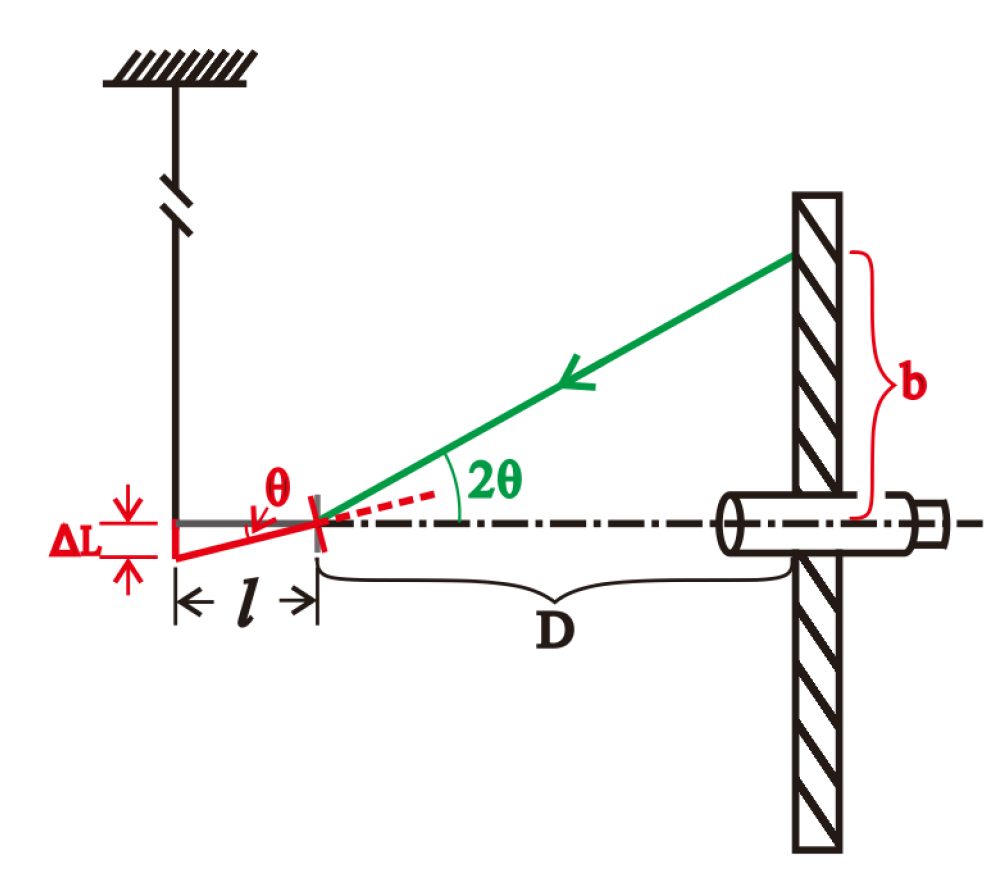
\includegraphics[width=5cm]{Figs/实验原理图.png}
    \caption{\small 实验原理图}
\end{wrapfigure}

材料受力后会发生形变,在弹性限度内,材料的应力和应变之比是一个常数,叫做
弹性模量,条形物体的沿纵向的弹性模量叫杨氏模量。它的大小标志了材料的刚性。
\begin{align}
    E=\dfrac{\dfrac{F}{S}}{\dfrac{\Delta L}{L}}=\frac{FL}{S\Delta L}
\end{align}
在样品截面积$S$上的作用应力为$F$,测量引起的相对伸长量$\dfrac{\Delta L}{L}$ ,即可计算出材料的杨氏模量$E$。因一般伸长量$\Delta L$很小,故采用光学放大法将其放大。光杠杆是一个带有可旋转的平面镜的支架,平面镜的镜面与三个足尖决定的平面垂直,其后足即杠杆的支脚与被测物接触。当杠杆支脚随被测物上升或下降微小距离$\Delta L$时,镜面法线转过一个微小的$\theta$角,而入射到望远镜的光线转过$2\theta$角,如图1所示:

根据图1和公式$(4)$可知:
\begin{align}
    \tan{\theta}&=\dfrac{\Delta L}{l}\approx\theta \\
    \tan{2\theta}&=\dfrac{b}{D}\approx2\theta
\end{align}
泰勒级数展开公式:
\begin{align}
    \tan{\theta}=\theta+\dfrac{\theta^3}{3}+\dfrac{2\theta^5}{15}+\dfrac{17\theta^7}{315}+\cdots,\quad\text{当}|\theta|<\dfrac{\pi}{2}
\end{align}
将公式$(2)$、$(3)$代入公式$(1)$中可以得到:
\begin{align}
    E=\dfrac{2DLF}{Slb}
\end{align}
其中:$L$为金属丝的长度,$D$为平面镜与直尺之间的距离,$l$为光杠杆的臂长,$b$为望远镜中所观察的到的标尺移动的距离,$S$为钢丝的截面积,通过测量钢丝的直径求得。

\section*{四、实验内容}

\begin{enumerate}
    \item 调节仪器
    \begin{enumerate}
        \item 调节放置光杠杆的平台与望远镜的相对位置,使光杠杆镜面法线与望远镜轴线大体重合。调节支架底脚螺丝,确保平台水平,调平台的上下位置,使管制器顶部与平台的上表面共面。
        \item 光杠杆的调节:光杠杆和镜尺组是测量金属丝伸长量的关键部件,光杠杆的镜面和足尖应平行,使用时足尖放在平台的沟槽内,后锥形足尖放在管制器的槽中,之后再调节平面镜的仰角使镜面垂直,即光杠杆镜面法线与望远镜轴线大体重合。
        \item 镜尺组的调节:调节望远镜、直尺和光杠杆三者之间的相对位置,使望远镜和光杠杆平面镜处于同等高度。要注意:按先粗调后细调的原则。利用望远镜上的准星瞄准光杠杆平面镜中的标尺像,使其能将标尺上的刻度反射到望远镜里,然后再细调。调节望远镜目镜视度圈,使目镜内分划板刻线清晰,再用手轮调焦使标尺像清晰。调节望远镜进行读数时要消除视差。如果没有找到标尺像,请不要过急调节调焦手轮,重新瞄准光杠杆平面镜中的标尺像,重复上述调试过程。
        \item 光杠杆、望远镜、标尺调整好以后,整个实验中防止位置变动。加减砝码要交叉轻放轻取避免晃动、倾斜,使钢丝与管制器之间发生摩擦,待钢丝静止后再读数。
    \end{enumerate}
    \item 测量
    \begin{enumerate}
        \item 测量钢丝长度,应注意两端点的位置,上端起于夹钢丝的两个半圆柱的下表面,下端止于管制器的上表面。
        \item 记录望远镜中标尺的读数作为钢丝的起始长度。在砝码托上逐次加$1kg$砝码(可加到$9kg$) ,观察每增加$1kg$时望远镜中标尺上的读数$r_i$,然后再将砝码逐次减去,记下对应的读数$r'_i$ ,取两组对应数据的平均值$\overline{r_i}$。
        \item 用米尺测量金属丝的长度$L$和平面镜与直尺之间的距离$D$,以及光杠杆的臂长$l$各$1$次。用千分尺测金属丝直径$d$,上、中、下各测$2$次,共$6$次,$0.570mm<d<0.620mm$。
    \end{enumerate}
    \item 逐差法:用逐差法处理数据得到$1kg$时对应的$b$值,并求$\dfrac{\Delta E}{E}$,给出$E$的最终表达式。$\Delta m=5\,g,\;\Delta L=0.05\,mm,\;\Delta D=0.05\,mm,\;\Delta l=0.05\,mm,\;\Delta b=0.05\,mm,\;\Delta d=0.001\,mm$
    \begin{align}
        \dfrac{\Delta E}{E}=\sqrt{\left(\dfrac{\Delta D}{D}\right)^2+\left(\dfrac{\Delta L}{L}\right)^2+\left(\dfrac{\Delta l}{l}\right)^2+\left(\dfrac{\Delta F}{F}\right)^2+\left(\dfrac{\Delta b}{b}\right)^2+\left(\dfrac{2\Delta d}{d}\right)^2}
    \end{align}
\end{enumerate}

\section*{五、数据记录}

原始数据见附录。

\section*{六、数据处理}

使用逐差法处理数据:
\begin{align*}
    L=853.8\;mm=0.8538\;m; \\
    D=1353.2\;mm=1.3532\;m; \\
    l=72.3\;mm=0.0723\;m.
\end{align*}

\begin{align*}
    b&=\dfrac{\sum_{n=1}^{4}(r_{i+4}-r_i)}{4\times4} \\
    &=\dfrac{(3.275-0.62+3.91-1.31+4.58-1.96+5.2-2.665)\;cm}{16}=0.651\;cm=6.51\times10^{-3}\;m \\
    S&=\dfrac{\pi\overline{d}^2}{4}=\dfrac{3.14\times(0.6055\;mm)^2}{4}=0.288\;mm^2=2.88\times10^{-7}\;m^2\quad \\
    F&=mg=1\;kg\times9.7887\;m/s^2=9.7887\;N\quad\dfrac{\Delta F}{F}=\dfrac{\Delta mg}{mg}=\dfrac{\Delta m}{m}=\dfrac{5\times10^{-3}\;kg}{1\;kg}=5\times10^{-3} \\
    E&=\dfrac{2DLF}{Slb}=\dfrac{2\times1.3532\;m\times0.8538\;m\times9.7887\;N}{2.88\times10^{-7}\;m^2\times0.0723\;m\times6.51\times10^{-3}\;m}=1.67\times10^{11}\;Pa=167\;GPa
\end{align*}

\begin{align*}
    \dfrac{\Delta E}{E}&=\sqrt{\left(\dfrac{\Delta D}{D}\right)^2+\left(\dfrac{\Delta L}{L}\right)^2+\left(\dfrac{\Delta l}{l}\right)^2+\left(\dfrac{\Delta F}{F}\right)^2+\left(\dfrac{\Delta b}{b}\right)^2+\left(\dfrac{2\Delta d}{d}\right)^2} \\
    &=\sqrt{\left(\dfrac{0.05\,mm}{1353.2\,mm}\right)^2+\left(\dfrac{0.05\,mm}{853.8\,mm}\right)^2+\left(\dfrac{0.05\,mm}{72.3\,mm}\right)^2+\left(5\times10^{-3}\right)^2+\left(\dfrac{0.05\,mm}{6.51\,mm}\right)^2+\left(\dfrac{2\times0.001\,mm}{0.6055\,mm}\right)^2} \\
    &=9.766\times10^{-3} \\
    \Delta E&=E\times\dfrac{\Delta E}{E}=1.67\times10^{11}\;Pa\times9.766\times10^{-3}=1.63\times10^9\;Pa\approx0.02\times10^{11}\;Pa \\
    E&=(1.67\pm0.02)\times10^{11}\;Pa \\
    U&=\dfrac{|E_{\text{测}}-E_{\text{真}}|}{E_{\text{真}}}=\dfrac{|1.67\times10^{11}\;Pa-2.00\times10^{11}\;Pa|}{2.00\times10^{11}\;Pa}\times100\%=16.5\%
\end{align*}

\section*{七、误差分析}

\begin{enumerate}
    \item 测量镜尺距离时米尺在空中悬空,无法保证完全拉直,可能会导致测量误差;
    \item 测量金属丝原长时,端点定位不准,米尺需要弯曲折叠才能测量,导致误差;
    \item 砝码轻微抖动和金属丝弹性滞后导致望远镜读数波动;
    \item 光杠杆未放平,导致微小误差;
    \item 望远镜并未固定死,触碰会有微小位移,导致误差。
\end{enumerate}

\section*{八、思考题}

利用光杠杆把测微小长度$\Delta L$变成测$b$,光杠杆的放大率为$\dfrac{D}{l}$,根据此式能否以增加$D$减小光杠杆臂长$l$,来提高放大率,这样做有无好处?有无限度?应怎样考虑这个问题?\\
答:

好处:放大率提高,微小形变更易观测,灵敏度增加,降低读数误差。

限度:增大$D$使得实验装置需更大空间,不便于操作;系统受外界振动或气流干扰导致的微小扰动都会放大,使最终读数不准确;减小$l$会导致相同拉力下光杠杆仰角$\theta$过大从而导致近似$\tan{\theta}=\theta$不适用。

综合来看,保证$\theta$足够小以确保近似有效,在实验条件允许范围内,平衡放大率与稳定性,选择适中的$D$和$l$。

\section*{九、实验结论}

经光杠杆放大法测得固体杨氏模量$E=(1.67\pm0.02)\times10^{11}\;Pa$,相对误差为:$16.5\%$

\end{document}